\documentclass[a4paper,11pt]{article}
\frenchspacing
\usepackage[T1]{fontenc}
\usepackage[utf8]{inputenc}
\usepackage[english]{babel}
\usepackage[pdftex]{graphicx}
\usepackage{hyperref}
\usepackage{amsmath,amssymb}
\usepackage{clock}
\usepackage{comment}
\usepackage{caption}
\usepackage{subcaption}
%\usepackage{subfigure}
\frenchspacing
\newcommand{\partder}[2]{\frac{\partial #1}{\partial #2}}
\newcommand{\der}[1]{\partial_{ #1}}
\newcommand{\ket}[1]{\left | {#1} \right \rangle }
\newcommand{\refstate}[0]{\textbf{0}}
\newcommand{\vacket}[0]{\ket{\refstate}}
\newcommand{\vacbra}[0]{\bra{\refstate}}
\newcommand{\bra}[1]{\left \langle {#1} \right | }
\newcommand{\ketbra}[1]{\ket{#1} \bra{#1}}
\newcommand{\innerprod}[2]{\left \langle {{#1} | {#2}} \right \rangle}
\newcommand{\uket}[0]{\ket{\uparrow}}
\newcommand{\dket}[0]{\ket{\downarrow}}
\newcommand{\ubra}[0]{\bra{\uparrow}}
\newcommand{\dbra}[0]{\bra{\downarrow}}
\newcommand{\hadj}[1]{{#1}^{\dagger}}
\newcommand{\conj}[1]{{#1}^{\ast}}
\newcommand{\cosine}[1]{\mathrm{cos}\left ( {#1}\right )}
\newcommand{\sine}[1]{\mathrm{sin}\left ( {#1}\right )}
\newcommand{\cosinep}[2]{\mathrm{cos}^{#2}\left ( {#1}\right )}
\newcommand{\sinep}[2]{\mathrm{sin}^{#2}\left ( {#1}\right )}
\newcommand{\expf}[1]{\mathrm{exp}\left ( {#1}\right )}
\newcommand{\determinant}[1]{\mathrm{det}\left ( {#1}\right )}
\newcommand{\trace}[1]{\mathrm{Tr}\left ( {#1}\right )}
\newcommand{\parent}[1]{\left( {#1} \right)}
\newcommand{\aver}[1]{ \left\langle  {#1}  \right\rangle }
\newcommand{\absval}[1]{\left| {#1} \right|}
\newcommand{\sset}[1]{\left\lbrace {#1} \right\rbrace }
\newcommand{\iden}[1]{\mathbf{1}_{#1}}
\newcommand{\ssum}[2]{\displaystyle\sum\limits_{#1}^{#2}}
\newcommand{\pprod}[2]{\displaystyle\prod\limits_{#1}^{#2}}
\newcommand{\commut}[2]{\left[ {#1} , {#2} \right]}
\newcommand{\acommut}[2]{\left\lbrace  {#1} , {#2} \right\rbrace }
\newcommand{\spann}[1]{\mathrm{span} \parent{{#1}}}
\newcommand{\ttrace}[2]{\mathrm{Tr}_{#1} \parent{#2}}
\newcommand{\logt}[1]{\mathrm{log_2} \parent{{#1}}}
\newcommand{\hilbert}[1]{\mathcal{H}_{{#1}}}
\newcommand{\genus}{g}
\newcommand{\gsfun}[0]{\eta_{GS}}
\newcommand{\vvec}[1]{\textbf{{#1}}}
\newcommand{\kk}[0]{\vvec{k}}
\newcommand{\tsection}[1]{\newpage \section{{#1}}}
\newcommand{\grad}[0]{\nabla}
\newcommand{\divv}[0]{\nabla \dot}
\newcommand{\curl}[0]{\nabla \times}
\newcommand{\vvar}[1]{\mathrm{var} \parent{{#1}}}
\newcommand{\bigo}[1]{\mathcal O \parent{{#1}}}
\newcommand{\qt}[0]{\tilde q}
\newcommand{\e}[1]{\times 10^{#1}}
\newcommand{\supremum}[1]{\mathop{\mathrm{sup}}_{{#1}}}
\newcommand{\nnorm}[2]{\absval{\absval{{#1}}}_{#2}}
\newcommand{\problem}[1]{\newpage \section*{{#1}}}
\newcommand{\hittime}[0]{\sigma_{\bar{\mathcal E}}}
\newcommand{\probb}[1]{\mathrm{P} \parent{{#1}}}
\newcommand{\expp}[1]{\mathrm{E} \parent{{#1}}}
\usepackage{tikz}
\usepackage{pgfplots}
\newcommand{\trans}[1]{{#1}^{\mathrm T}}
\newcommand{\indicatorfun}[1]{\mathbf{1}_{#1} }

\newcommand{\taubar}{\bar{\sigma}_{\bar{\mathcal E}}}

% used only for something irrelevant

\newcommand{\sthnolla}[0]{}

\title{tex notes}
\author{Juho Happola}
\begin{document}

\section*{Variance reduction by importance sampling}

\subsection*{a}
Suppose we want to compute $\alpha \equiv \expp{g \parent{W}}$
with g non-negative and $W \sim f_W$. Let $X$ be a random variable
$X \sim f_X$, then
\begin{align}
\alpha = \expp{g \parent{X} \frac{f_W \parent{X}}{ f_X \parent{X}}}.
\end{align}
Proof:
\begin{align}
\alpha =& \int_{\mathbb R} g \parent{x} f_W \parent{x} dx
\\
=& 
\int_{\mathbb R} g \parent{x} \frac{ f_X \parent{x} }{ f_X \parent{x} } f_W \parent{x} dx
\\
=& 
\int_{\mathbb R} g \parent{x} \frac{ f_W \parent{x} }{ f_X \parent{x} } f_X \parent{x} dx
\\
=& \expp{g \parent{X} \frac{ f_W \parent{X} }{ f_X \parent{X} } }.
\end{align}

\subsection*{b,c}
The above result allows solving $\alpha$ by Monte Carlo (MC) methods.
When we sample from distribution $f_X$ to estimate $\alpha$,
the mean square error (MSE) of the MC estimator 
\begin{align}
\mathrm{MSE} \propto \int_{\mathbb R}  \parent{ \parent{g\parent{x} \frac{f_W}{f_X} \parent{x}}^2 - \alpha^2 }  f_X \parent{x} dx.
\end{align}
The integrand is zero by choosing $f_X \parent{x}=f_X^* \parent{x} = \frac{f_W \parent{x} g \parent{x}}{\alpha}$, and thus
the variance of the MC estimator is minimised by choosing $f_X=f_X^*$. In practice, this result is of little significance,
since if we knew the exact value of $\alpha$, there would be no need for the MC estimator in the first place.

\subsection*{d}
Suppose we wish to evaluate $\probb{\mathcal N \parent{0,1} >3.75}$.
The naive MC estimator would be given by $g \parent{x} = \mathbf 1_{x>\frac{15}{4}} \parent{x}$ and
$f_W \parent{x} = \sqrt{2 \pi } \expf{-\frac{x^2}{2}}$. Alternatively, using an affine change
of variables,
we may choose for any $\delta \in \mathbf R$: $g_\delta \parent{x} = \mathbf 1_{x>\frac{15}{4}+\delta}$
and $f_W = \sqrt{2 \pi } \expf{-\frac{\parent{x-\delta}^2}{2}}$ and obtain the correct result.

In order to use the MC estimate, we need to be able to sample numbers, from
the distribution $\mathcal N \parent{\delta,1}$. And evaluate $g$ for each of those realisations.
An example implementation of this is given in \url{https://github.com/Virtakuono/SME_HW3_Example/blob/master/examples.py}
The MC estimator is given by:
\begin{align}
\overline \alpha = \ssum{m =1}{M} \frac{g_\delta \parent{X}}{M},
\end{align}
with $X_m \sim  N \parent{\delta,1}$ i.i.d. In the example we set $\delta=2$.
Since $\expp{X_m} = \delta$, $\expp{\overline \alpha} = \alpha$. Central
limit theorem guarantees that $\overline \alpha$ is approximately normally
distributed. To estimate the confidence interval, we compute the sample variance
as
\begin{align}
\overline \sigma^2 = \ssum{m=1}{M} \frac{\parent{g_\delta \parent{x}- \overline \alpha}}{M-1}.
\end{align}

Let
\begin{align}
\Phi_{\mu,\sigma} \parent{z} = \parent{ 2 \pi \sigma^2}^{-1}  \int_{-\infty}^z \expf{\frac{\parent{x-\mu}^2}{2 \sigma^2}}.
\end{align}
Then, there are ready implementations for the inverse of $\Phi_{\mu,\sigma}$, that
allow us to compute $z^*$ such that $\Phi_{0,1} \parent{z^*} = 0.95$. Using this
together with the fact that our MC estimator is approximately normally distributed,
we set $\eta = z^* \sqrt{\frac{\overline \sigma^2}{M}}$ and obtain the confidence interval
$[\overline \alpha - \eta, \overline \alpha + \eta]$. For the precise results, see table
\ref{tb:impsamp}.

\begin{table}
\begin{center}
\begin{tabular}{c c c}
M & $M=10^4$ & $M=10^5$ \\
\hline
Naive MC & $[0.000000,0.000433]$ (116 \%) &$[0.000055,0.000165]$ (50 \%) \\
Refined MC &$ [0.000084,0.000090]$ (3\%) &$ [0.000088,0.000089]$ (1\%) \\
Exponential & $[0.000086,0.000103]$ (9\%) & $ [0.000085,0.000091]$ (3\%)
\end{tabular}
\end{center}
\caption{\label{tb:impsamp}
Confidence intervals for the MC estimators and relative
errors when sampling from $\mathcal N \parent{0,1}$
and from $\mathcal N \parent{5.75,1}$.
Note that the reference value is $\Phi \parent{5.75} =0.000088$
so that there is almost 40\% that none of the realisations of of a
random sample of $M=10^4$ exceed $5.75$, leading to an estimate
of zero, and vanishing variance.
}
\end{table}

\subsection*{e}
We may, of course, use an exponential density too.
To ensure that half of the samples generated exceed 5.75, we
may set
\begin{align}
\lambda = \frac{\mathrm{ln} 2}{5.75}.
\end{align}.
Further improvements can naturally be made, optimising over $\lambda$ as well
as making affine transformation of the random variable.

\section*{Generate non-uniformly distributed random numbers given uniform}

\subsection({a}

A mean zero unit variance random variable $X$ has a Laplace distribution if its pdf is $f(x) = \frac{1}{2}  e^{-|x|}$.\\
\textbf{Algorithm} to generate such random variable:
\vspace{0.02in}
\begin{itemize}
\item $u \sim U(0,1)$
\item $ X \sim F_{U}^{-1}(u)$, where 
\begin{equation*}
 F_{X}(x) =
  \begin{cases}
   1 - \frac{1}{2} e^{-x},\, x \geq 0 \\
   \frac{1}{2} e^{-x},\,    x < 0
  \end{cases}
\end{equation*}
\begin{equation*}
 F^{-1}_{U}(u) =
  \begin{cases}
   \log{(2u)}, \,     0< u \leq \frac{1}{2} \\
   -\log{(2(1-u))} ,  \,  \frac{1}{2} \leq u < 1.
  \end{cases}
\end{equation*}
\end{itemize}

\subsection*{b}

 Algorithm to generate $Y \sim N(\mu,\sigma)$ random variables using the result above.\\
Assume that there exists $\epsilon \in (0,1]$ such that $\epsilon \frac{f_{Y}(X_k)}{f_{X}(X_k)} \leq 1$.
\textbf{Algorithm} (Acceptance-Rejection)
\vspace{0.02in}
\begin{itemize}
\item Set k=1
\item Sample two independent random variables $X_k$ and $U_k \sim U(0,1)$
\item If $U_{k} \leq \epsilon \frac{f_{Y}(X_k)}{f_{X}(X_k)}$, then accept $Y = X_k$ as sample from $N(\mu,\sigma)$. Otherwise, reject $X_k$, increment k by $1$ and go back to previous step.
\end{itemize}

\subsection*{c}
 Let $U$ and $V$ be two independent standard Gaussian random variables. Prove that the ratio $\frac{U}{V}$ is a Cauchy random variable.\\
\textbf{Proof}
\vspace{0.02in}
%The joint pdf of $U$ and $V$ is $f_{UV} (u,v) = \frac{1}{2\pi} e^{-\frac{u^2 + v^2}{2}}$.\\
Let $Z = \frac{U}{V}$ then cdf of $Z$ is given by
\begin{eqnarray*}
F_{Z}(z) &=& P(\frac{U}{V} \leq z), \\
&=& P(U \leq zV | V>0) + P(U \geq zv | V < 0), \\
&=& \int_{0}^{\infty} \left( \int_{-\infty}^{zv} f_{U}(u) \right) f_{V}(v) dv + \int_{-\infty}^{0} \left( \int_{zv}^{-\infty} f_{U}(u) \right) f_{V}(v) dv.
\end{eqnarray*}
Then, the pdf of $Z$ is given by
\begin{eqnarray*}
f_{Z}(z) &=& \frac{dF_{Z}(z)}{dz}, \\
&=& \int_{0}^{\infty} v f_{U}(zv) f_{V}(v) dv + \int_{-\infty}^{0} v f_{U}(zv) f_{V}(v) dv, \\
&=& 2 \int_{0}^{\infty} v f_{U}(zv) f_{V}(v) dv = \frac{1}{\pi(1+z^2)}
\end{eqnarray*}

\subsubsection({Algorithm}
\begin{itemize}
\item Generate samples from independent standard Gaussian random variables U and V.
\item Compute the samples $Z = \frac{U}{V}$.
\end{itemize}

\section*{Kernel Density Estimator (KDE)}

\subsection*{a}

We propose to estimate
a density function $\rho \parent{y}$
based on a MC sample of realisations $y_i \in \mathbb R^d$
from the density $\rho$ as follows
\begin{align}
\hat \rho \parent{y} = \frac{1}{M h^{-d}} \ssum{m=1}{M} K \parent{\frac{y-y_i}{h}},
\end{align}
with
\begin{align}
K \parent{x} = 2^{-d} \mathbf 1_{\nnorm{x}{L_2}} \parent{x}
\end{align}

In this estimation, we commit two errors.

\subsubsection*{bias error}

\begin{align}&\rho \parent{u} - \expp{\hat \rho \parent{y}}
\\
=& 
\rho \parent{y }
\int_{\mathbb R^d} h^{-d} K \parent{\frac{y-z}{h}} \rho \parent{z} dz
\\
=& \int_{\mathbb R^d} \parent{\rho \parent{y}- \rho \parent{y-h z}}  K\parent{z} dz
\\
\approx & 
\int_{\mathbb R^d}
\parent{\rho \parent{y} - \parent{\rho \parent{y} - h z_i \partial_{y_i} \rho \parent{y} + h^2 z_i z_j \partial_{z_i,z_j}^2 \rho \parent{y} }}
K \parent{z}
dz
\\
= & \frac{h^2}{2}  \partial_{y_i y_j} \rho \parent{u} \int_{\mathbb R^d} z_i z_j K \parent{z}  dz \propto h^2
\end{align}

\subsubsection*{statistical error}

The variance is bounded by
\begin{align}
\mathrm{V} \parent{K \parent{\frac{y-z}{h}}} \leq \expp{K^2 \parent{\frac{y-z}{h}}}
\end{align}
and
\begin{align}
\expp{K^2 \parent{\frac{y-z}{h}}}
\approx
\int_{\mathbb R^d}
K^2 \parent{z} h^d \parent{\rho \parent{y} - h z_i \partial_{y_i} \rho \parent{y} + \frac{h^2}{2} z_i z_j \partial_{y_i y_j}^2 \rho \parent{y} }
dz,
\end{align}
thus
\begin{align}
\mathrm{V} \parent{\hat \rho \parent{y}}
=& M^{-1} h^{-2d} \mathrm{V} \parent{K \parent{\frac{y-z}{h}}}
\\
\geq& M^{-1} h^{-2d} h^{d} \rho \parent{y} \int_{\mathbb R^d} K^2 \parent{z} dz
\propto M^{-1} h^{d}
\end{align}

\subsubsection*{Total error}
With undefined constants $A$ and $B$ we have that the 
total error squared (TSE) is given as
\begin{align}
\mathrm{TSE} \approx A h^4 + \frac{B}{Mh^d}.
\end{align}
The critical point of the total square error
is thus given by
\begin{align}
h^{4+d} \propto M^{-1}.
\end{align}
This choice implies that the bias and sampling errors are of the same order
\begin{align}
\mathrm{TSE} = \bigo{M^{-\frac{2}{d+4}}}
\end{align}

With the above analysis, we produce the set of three images (\ref{fig:1ddens})
for varying $M$ for a one-dimensional KDE and an example of
two-dimensional gaussian example (\ref{fig:2ddens}).

\begin{figure}
\begin{center}
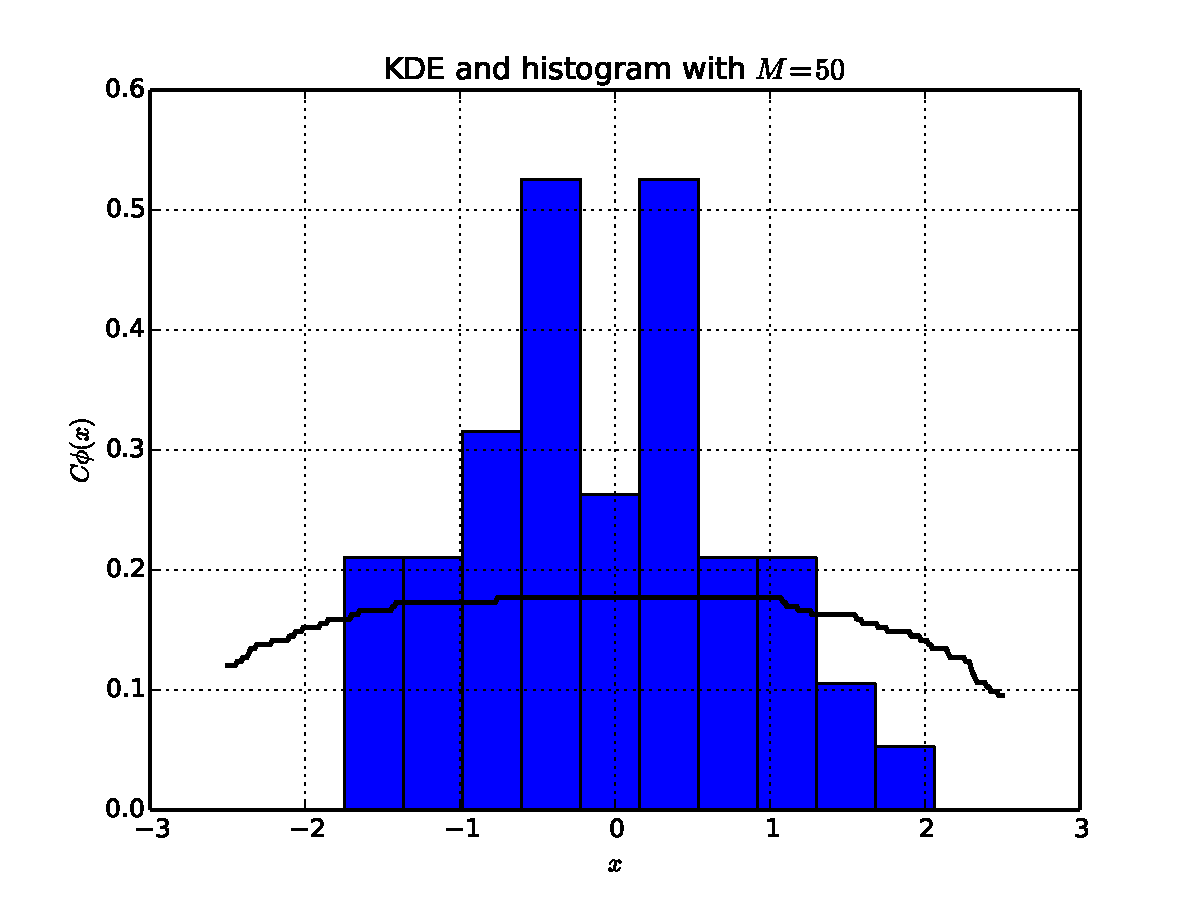
\includegraphics[width=40mm]{./kde_histogram_M_50.pdf}
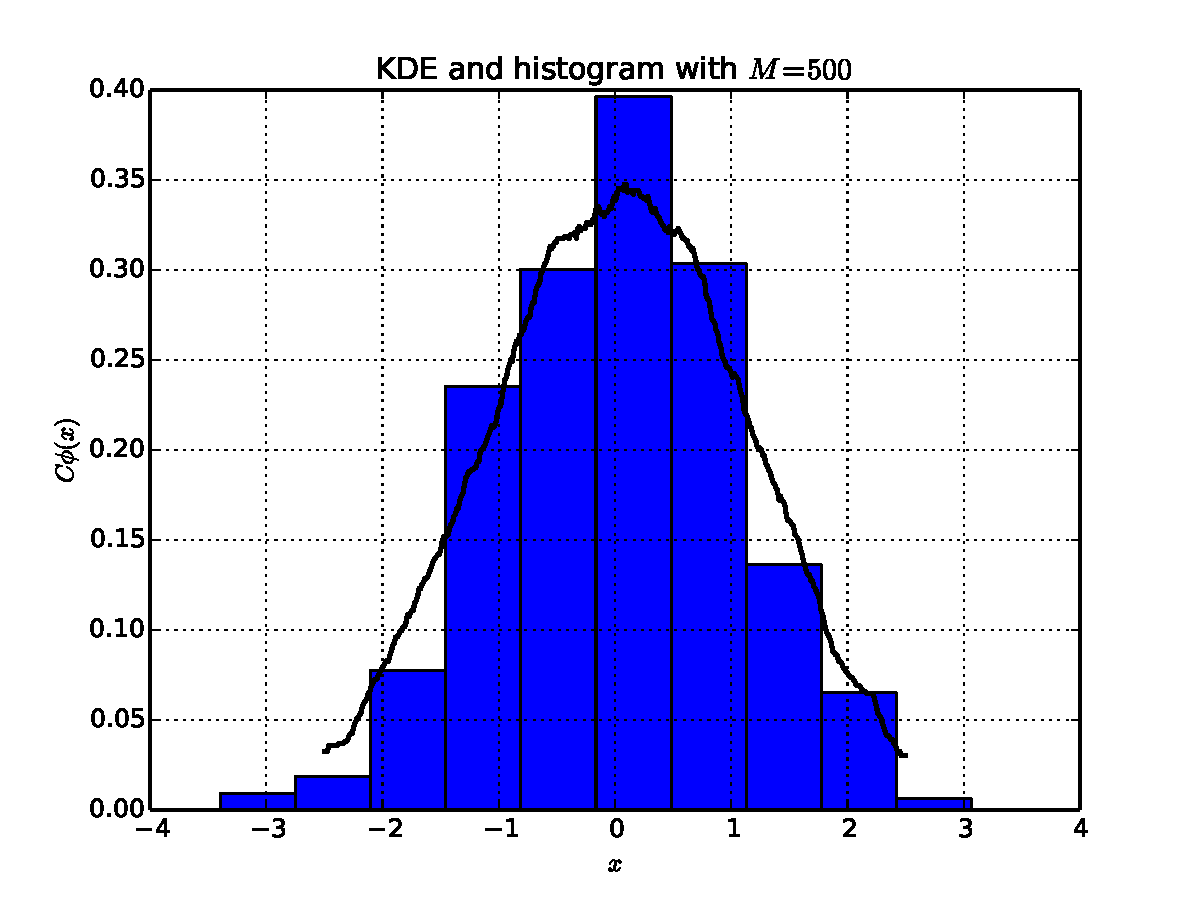
\includegraphics[width=40mm]{./kde_histogram_M_500.pdf}
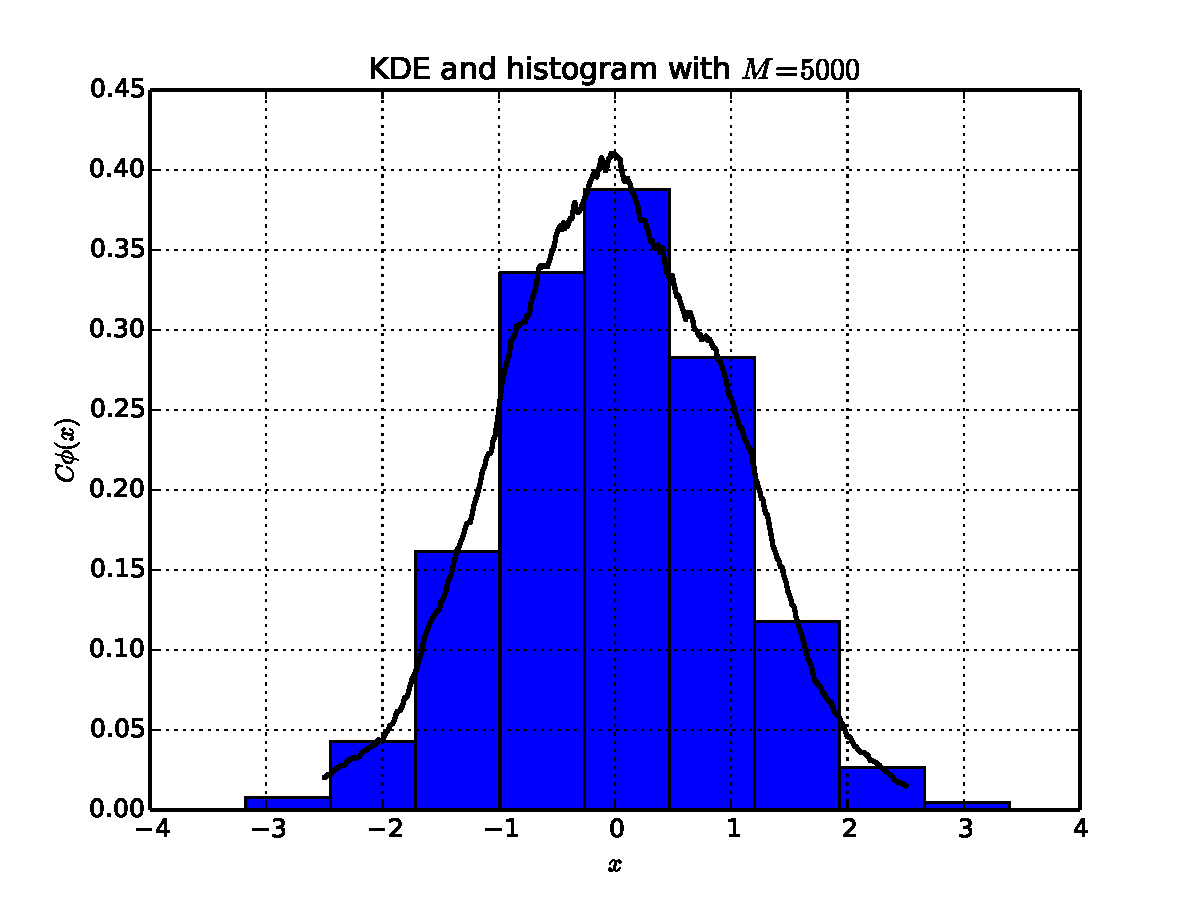
\includegraphics[width=40mm]{./kde_histogram_M_5000.pdf}

\caption{
\label{fig:1ddens}
One-dimensional multivariate Gaussian and corresponding
KDEs.
}
\end{center}
\end{figure}

\begin{figure}
\begin{center}
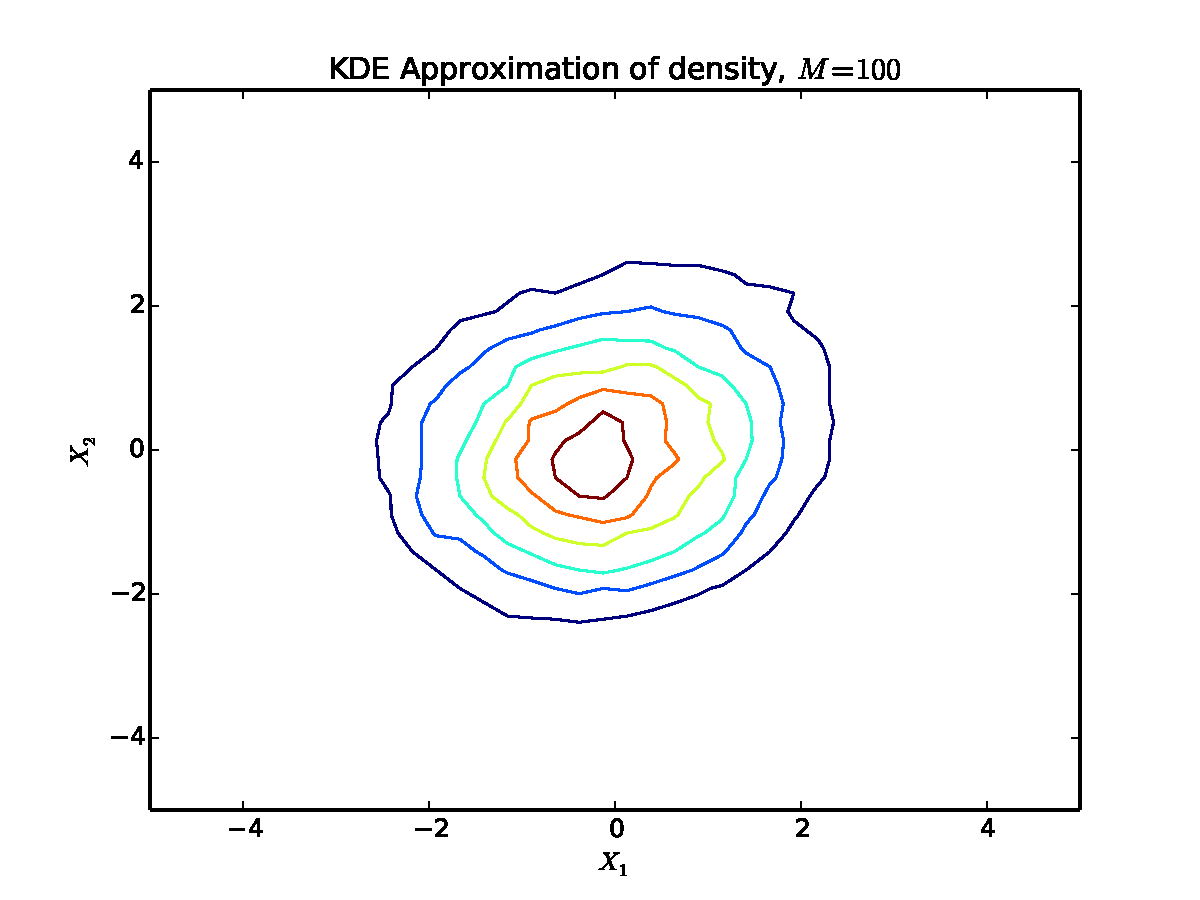
\includegraphics[width=60mm]{./approximation.pdf}
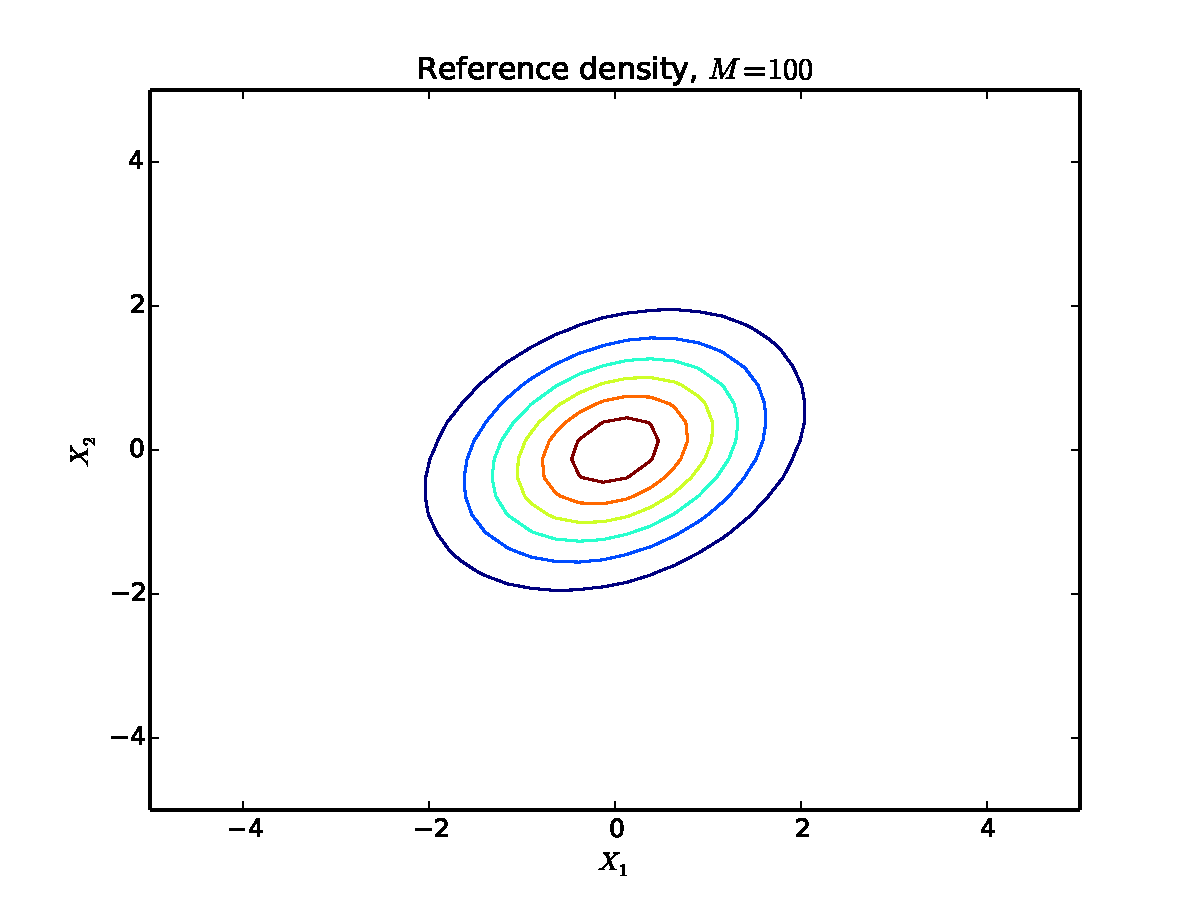
\includegraphics[width=60mm]{./reference.pdf}
\caption{
\label{fig:2ddens}
Two-dimensional multivariate Gaussian estimated (left) and exactly computed (right).
$M=100$ samples, $h=0.5$ 
}
\end{center}
\end{figure}

\section*{KDE for conditional expectation}

\subsection*{a}

Consider the Nadaraya-Watson estimator (cf. \cite{kdecond}) $\hat{g}(x)$ for $E[Y|X=x]$ which is derived as follows:
%\vspace{0.02in}
\begin{equation*}
g(x) = E[Y|X=x] = \frac{\int y f(y,x) dy}{f(x)},
\end{equation*}
using the KDE for both $f(y,x)$ and $f(x)$
\begin{eqnarray*}
\hat{f}(y,x) &=& \frac{1}{n} \sum_{i = 1}^{n} \kappa_{h}(y - Y_i) \kappa_{H}(x - X_i), \\
\hat{f}(x) &=& \frac{1}{n} \sum_{i = 1}^{n} \kappa_{H}(x - X_i),
\end{eqnarray*}
and the fact that $\int z\kappa_{h} (z)dz = 0$, we obtain
\begin{equation*}
\hat{g}(x) = \frac{ \sum_{i = 1}^{n}\kappa_{H}(x - X_i) Y_{i}}{\sum_{i = 1}^{n} \kappa_{H}(x - X_i)}.
\end{equation*}

Optimal rate of convergence\\
Note we have
\begin{eqnarray*}
Y_i &=& g(X_i) + \epsilon_i, \\
Y_i &=& g(x) + (g(X_i) - g(x)) + \epsilon_i,
\end{eqnarray*}
where $E(\epsilon_i | X_i) = 0$ and $E(\epsilon^2_i | X_i = x) = \sigma^2(x)$. \\
Therefore, the estimator can be written as
\begin{equation*}
\hat{g}(x) = g(x) + \frac{\hat{m}_{1}(x)}{\hat{f}_{X}(x)} + \frac{\hat{m}_{2}(x)}{\hat{f}(x)},
\end{equation*}
where
\begin{eqnarray*}
\hat{m}_{1}(x) &=&  \frac{1}{n} \sum_{i = 1}^{n} \kappa_{H}(x - X_i)  (g(X_i) - g(x)), \\
\hat{m}_{2}(x) &=&  \frac{1}{n} \sum_{i = 1}^{n} \kappa_{H}(x - X_i)  \epsilon_i.
\end{eqnarray*}

If $d=1$, we can show that
\begin{eqnarray*}
E(\hat{m}_{1}(x)) &=& \frac{1}{h} \int k \left( \frac{x-u}{h} \right) (g(u) - g(x)) f(u) du\\
&=& \int k(z) (g(x+hz) - g(x)) f(x+hz) dz\\
&& \text{(Taylor expansion)} \\ 
&=& h^2 B(x) f(x) \int k(z) z^2 dz + o(h^2),
\end{eqnarray*}
where $B(x) = \frac{1}{2} g''(x) + \frac{g'(x)}{f(x)} f'(x)$.\\
Similarly, we can obtain $Var( \hat{m}_{1}(x)) = O(\frac{1}{nh})$.

\begin{eqnarray*}
E(\hat{m}_{2}(x)) &=& 0, \\
Var(\hat{m}_{2}(x)) &=& \frac{1}{nh^2} \int k \left( \frac{x-u}{h} \right)^2  \sigma^2(u) f(u) du \\
&=& \frac{1}{nh} \int  k(z) \sigma^2(x+hz) f(x+hz) dz \\
&& \text{(Taylor expansion)} \\
&=& \frac{\sigma^2(x)f(x)}{nh}  \int k(z)^2 dz + o(h^2),
\end{eqnarray*}
The asymptotic mean square error( AMSE ) when $d= 1$ is
\begin{equation*}
\left( h^{2} B(x) \right)^{2} \left( \int k(z) z^{2} dz \right)^{2} +  \frac{ \sigma(x)^{2} f_{X}(x)}{nh}  \left( \int k(z)^2 dz \right).
\end{equation*}


In General, the asymptotic mean square error( AMSE ) is given by
\begin{equation*}
\left( \sum_{j=1}^{d} h_{j}^{2} B_{j}(x) \right)^{2} \left( \int k(z) z^{2} dz \right)^{2} +  \frac{ \sigma(x)^{2} f_{X}(x)}{n|H|}  \left( \int k(z)^2 dz \right)^{d},
\end{equation*}
where $B_{j}(x) = \frac{1}{2} \partial^{2}_{x_j} g(x) + f(x)^{-1} \partial_{x_j} g(x) \partial_{x_j}f(x)$ 
and the optimal value for $h$ is proportional to $N^{-\frac{1}{d+4}}$.

\subsection*{b}

Let us reuse the sample from the last exercise and show an illustration
of the performance of the algorithm in figure \ref{fig:cond}

\begin{figure}
\begin{center}
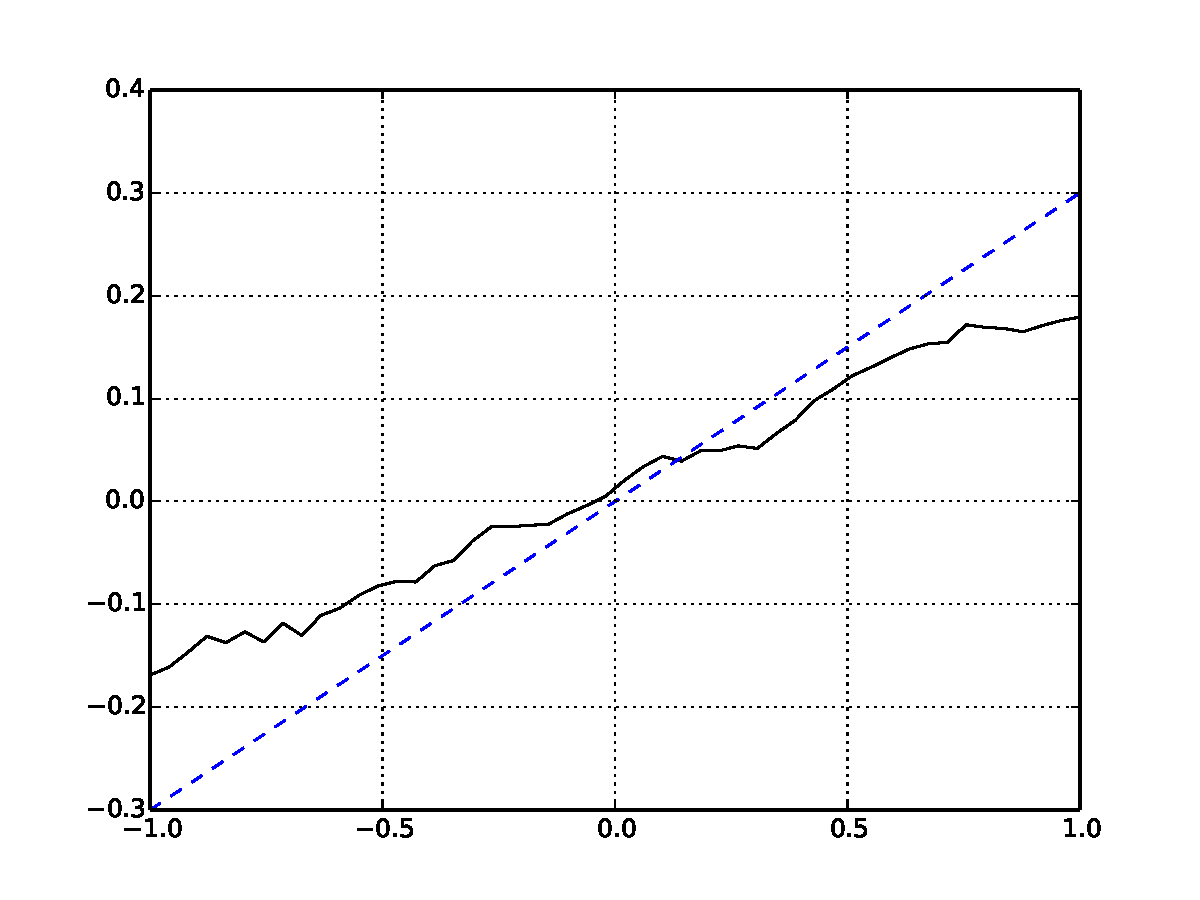
\includegraphics[width=80mm]{./cond.pdf}
\end{center}
\caption{
\label{fig:cond}
The conditional expectation of $y$, given $x$. The sample data is
generated from $M=400$ realisations of i.i.d. Gaussian random
variables $z_1$ and $z_2$. $x_2=z_2$, $x_1=z_1+0.3z_2$.
The blue dashed line indicates the reference at slope $0.3$.
}
\end{figure}

\section*{Monte Carlo and Variance Reduction}

The task at hand is to evaluate an option on an underlying that is an arithmetic
mean of a log-normal random variable. No closed form solution exists. However,
we do have a closed form expression for the arithmetic mean of normal variables.
Based on a visual inspection (cf. fig \ref{fig:loghist}), the distribution of the underlying is, however, somewhat
close to a Gaussian and especially the relevant part, the right tail of the distribution could 
be approximated with a Gaussian with a decent fidelity.
\begin{figure}
\begin{center}
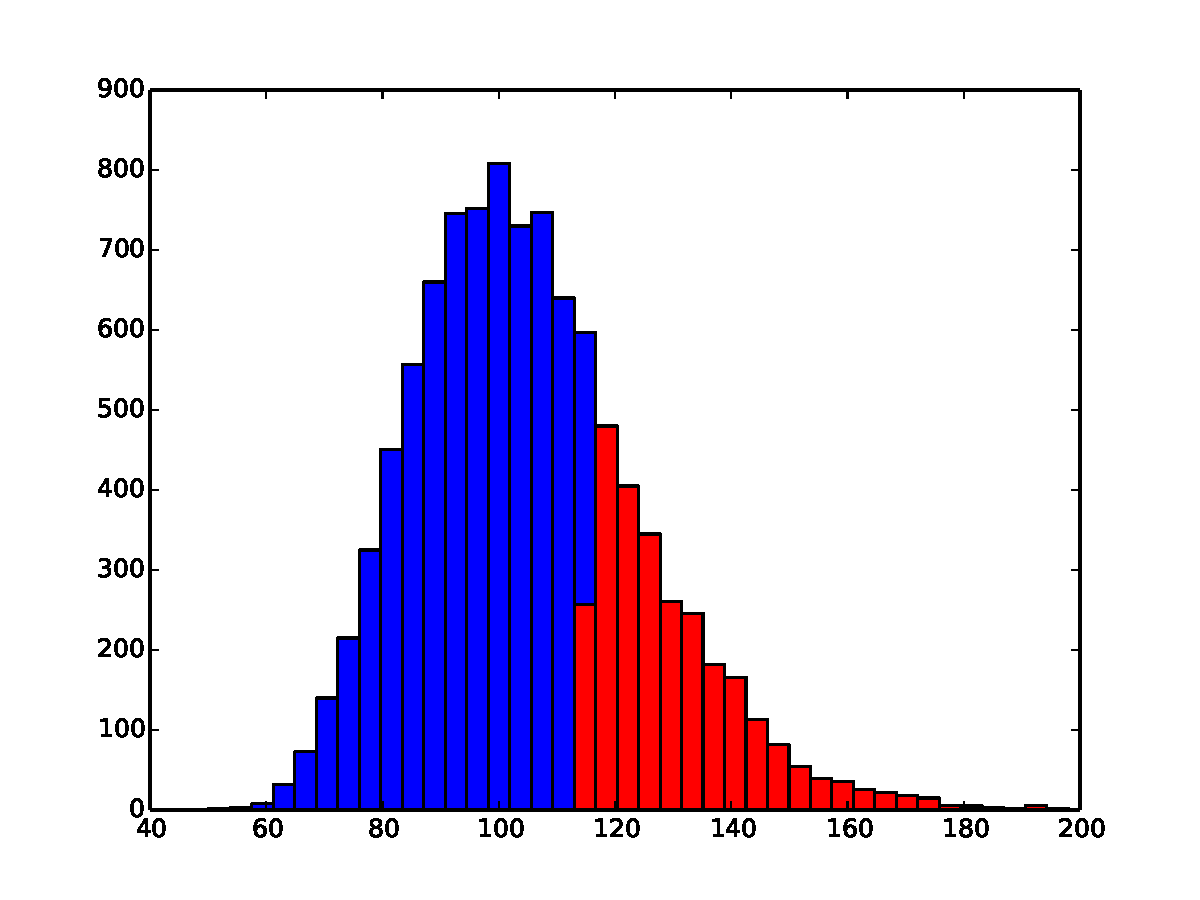
\includegraphics[width=60mm]{./v_n_histogram.pdf}
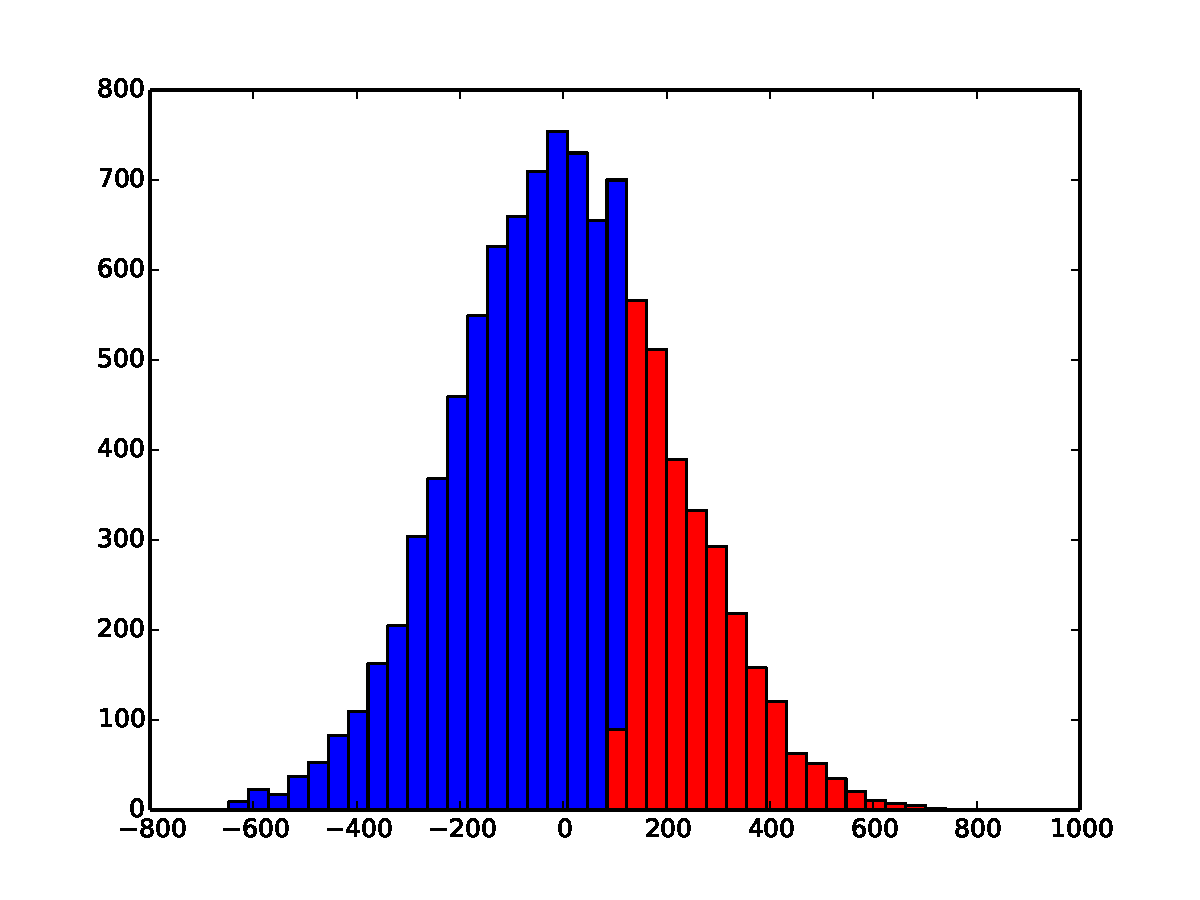
\includegraphics[width=60mm]{./v_n_histogram_cv.pdf}
\end{center}
\caption{
\label{fig:loghist}
The distribution of the underlying of the Asian Option (left)
and a control variate (right). The right tail of the distribution is
coloured left to indicate
realisations \emph{in the money} with strikes $K$  and $\tilde K$.
}
\end{figure}
We have
\begin{align}
V_N=V_0 \pprod{n}{N} R_n.
\end{align}
Empirically, we see that the probability $P_{otm}$ of $V_N$ being out of the money is
approximately 72 per cent.
Define
\begin{align}
Q = \ssum{n=1}{N} \parent{50-n} \parent{\mathrm{ln}~R_n - r \Delta t},
\end{align}
we note that both $Q$ and $V_N$ are increasing in all the random variables
$R_n$. Furthermore, we know that $Q$ entered and normally distributed with
$\tilde \sigma^2 = \ssum{n=1}{N} \parent{50-n}^2$. With the inverse cumulative distribution
$\Phi^{-1}$ we can define
\begin{align}
\tilde K = \tilde \sigma \Phi^{-1} \parent{P_{otm}}.
\end{align}
Then our control variate is
\begin{align}
G=\parent{Q-\tilde K}^+.
\end{align}
We have
\begin{align}
\int_{-\infty}^{\infty} \frac{1}{\sqrt{2 \pi}} \expf{-\frac{x^2}{2 \tilde \sigma^2}} \parent{x-k}^+
 =
 \frac{\tilde \sigma}{\sqrt{2 \pi}}
 \expf{-\frac{k^2}{2 \tilde \sigma^2}}
 +k \parent{\Phi \parent{k} -1}.
\end{align}
We have that the correlation coefficient $\rho$ between 
$G$ and $C = \parent{\ssum{n=1}{N}\frac{V_n}{K}-K,0}^+$
exceeds 0.99, see fig \ref{cvfig}.
\begin{figure}
\begin{center}
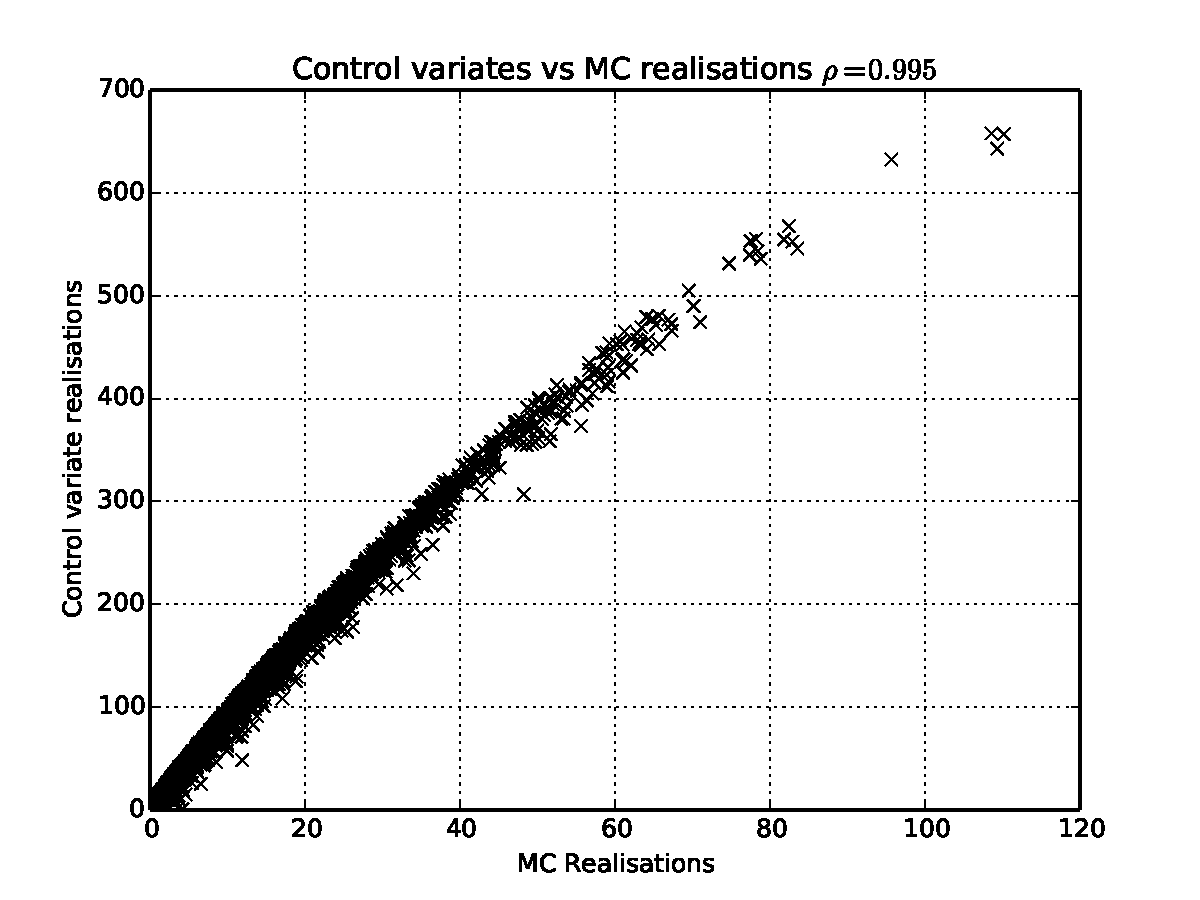
\includegraphics[width=100mm]{./cvplot.pdf}
\end{center}
\caption{
\label{cvfig}
The MC realisations and corresponding
control variates show a near-perfect correlation
}
\end{figure}

We can form the estimators
\begin{align}
\overline C_1 =& \ssum{m=1}{M} \frac{ \parent{\parent{ \ssum{n=1}{N} V_0 \pprod{m=1}{n} R_n}-K}^+ }{M}
\\
\overline C_2 =& \ssum{m=1}{2M} \frac{ \parent{\parent{ \ssum{n=1}{N} V_0 \pprod{m=1}{n} \tilde R_{n,m}}-K}^+ }{M} + 
 \ssum{m=1}{2M} \frac{ \parent{\parent{ \ssum{n=1}{N} V_0 \pprod{m=1}{n} \tilde R_{n,m}}-K}^+ }{M}
 \\
 \overline C_3 =& \ssum{m=1}{M} \frac{ \parent{\parent{ \ssum{n=1}{N} V_0 \pprod{m=1}{n} R_n}-K}^+  + \beta \parent {G_m - \expp{Q}}}{M}
\\
\overline C_4 =& \ssum{m=1}{2M} \frac{ \parent{\parent{ \ssum{n=1}{N} V_0 \pprod{m=1}{n} R_n}-K}^+  + \beta \parent{G_m - \expp{Q}}}{M}
\nonumber
\\
& \ssum{m=1}{2M} \frac{ \parent{\parent{ \ssum{n=1}{N} V_0 \pprod{m=1}{n} R_n}-K}^+  + \beta \parent{Q_m - \expp{Q}}}{M},
\end{align}
for the plain vanilla, antithetic, control variate, and combination methods, respectively. The
$R_{n,m}$ are understood to be independent realisations of the incrementation for $n$th time step
for realisation $m$ The antithetic variables
are defined as
\begin{align}
\tilde{R}_{n,m} = \expf{-\log{R_{n,m}+\Delta t r}}
\end{align}
and
\begin{align}
\tilde{Q}_m &= \ssum{n=1}{N} \parent{50-n} \parent{\mathrm{ln}~ \tilde{R}_{nm} - r \Delta t},
\\
G_m&=\parent{Q_m-\tilde K}^+
\\
\tilde G_m&=\parent{\tilde Q_m-\tilde K}^+.
\end{align}

In order to minimise the variance of the estimators, we set $\beta = \rho \sqrt{\frac{\sigma_C^2}{\sigma_Q^2}}$
with $\sigma_C^2$ being the variance of the plain vanilla MC realisations and $\sigma_Q^2$ the variance of
the control variate realisations. With $M=10000$, we obtain the results in table \ref{tb:MC}:
\begin{table}
\begin{center}
\begin{tabular}{c c cc }
  Plain vanilla & Antithetic & Control variate & Hybrid \\
  \hline
0.15 \% & 0.10 \% & 0.012 \% & 0.0085 \% 
\end{tabular}
\end{center}
\caption{\label{tb:MC}
Widths of 95 \% confidence bands for different Monte Carlo estimators for $M=1000$.
Modified option price approximately $4.3$.
}
\end{table}
The exact computational cost of each estimator depends on how computationally costly
it is to generate time steps compared to the cost of generating random numbers. For a
rough approximation, we may state that the computational cost of the antithetic and
control variate estimators are twice that of the plain vanilla and the hybrid method requires four-fold
computational effort.

\section*{Confidence interval, Bootstrapping}

In order to compute the expected shortfall we reuse the MC sample from the previous exercise.
Let our MC estimator $\overline C$ be given as:
\begin{align}
\overline C = \ssum{m=1}{M} \frac{X_i}{M}.
\end{align}
Then let us draw $N\times M, ~ N,M \in \mathbb Z$ random variables
$k_i \in \sset{1,2,3,...M}$. Then define $S_j$ such that
\begin{align}
\# A_j =\# \sset{k_i: X_{k_i}>S_j, \parent{j-1 }M \leq i \leq jM-1} = \lfloor pM \rfloor
\end{align}
for $j \in {1,2,3,4,...,N}$. and
\begin{align}
Q _j = \ssum{i \in A_j}{} \frac{X_i \mathbf{1}_{x>S_j} \parent{X_i}}{\# A_j}
\end{align}
then the estimated confidence interval can be noted as $[Q^-,Q^+]$
as
\begin{align}
\# \sset{j: Q_j<Q^{-}} =& \left \lfloor \frac{qN}{2} \right \rfloor \\
\# \sset{j: Q_j<Q^{+}} =&  \left \lfloor \frac{qN}{2} \right \rfloor .
\end{align}
Setting $N=1000$, we obtain the results in the table \ref{tb:BS}

\begin{table}	
\begin{center}
\begin{tabular}{c c c c }
  $p$ & $0.9$  & $0.95$  &  $0.99$ \\
  \hline
Confidence interval & $[28.28, 30.01]$ & $[36.51, 38.80]$ & $[52.34, 57.68]$ 
\end{tabular}
\end{center}
\caption{\label{tb:BS}
Confidence intervals for the Expected Shortfall for problem 5 example
for various quantiles.
The width of the confidence interval tends to increase as a function of $q$.	
}
\end{table}

\begin{thebibliography}{9}

\bibitem{kdecond} Nadaraya-Watson estimator - \url{http://www.maths.manchester.ac.uk/~peterf/MATH38011/NPR\%20N-W\%20Estimator.pdf}

\bibitem{thecode} Example code in python. \url{https://github.com/Virtakuono/SME_HW3_Example/blob/master/examples.py}
\end{thebibliography}

\end{document}